\documentclass[11pt]{article}
\usepackage[margin=1in]{geometry}
\usepackage{enumitem}
\usepackage{hyperref}
\usepackage{graphicx}
\usepackage{array}
\usepackage{multicol}
\usepackage{longtable}
\usepackage{titlesec}
\usepackage{amsmath} 
\usepackage{amssymb}
\usepackage{float}
\usepackage{listings}
\usepackage{xcolor}

\definecolor{codegreen}{rgb}{0,0.6,0}
\definecolor{codegray}{rgb}{0.5,0.5,0.5}
\definecolor{codepurple}{rgb}{0.58,0,0.82}
\definecolor{backcolour}{rgb}{0.95,0.95,0.92}

\lstset{
    backgroundcolor=\color{backcolour},   
    commentstyle=\color{codegreen},
    keywordstyle=\color{magenta},
    numberstyle=\tiny\color{codegray},
    stringstyle=\color{codepurple},
    basicstyle=\ttfamily\footnotesize,
    breakatwhitespace=false,         
    breaklines=true,                 
    captionpos=b,                    
    keepspaces=true,                 
    numbers=left,                    
    numbersep=5pt,                  
    showspaces=false,                
    showstringspaces=false,
    showtabs=false,                  
    tabsize=2
}

\titleformat{\section}{\large\bfseries}{\thesection}{1em}{}
\titleformat{\subsection}{\normalsize\bfseries}{\thesubsection}{1em}{}

\begin{document}

\begin{center}
    \large \textbf{Sri Sivasubramaniya Nadar College of Engineering, Chennai} \\
    (An autonomous Institution affiliated to Anna University) \\
    \vspace{0.3cm}
\end{center}

\begin{table}[H] 
\renewcommand{\arraystretch}{1.5}
\resizebox{\textwidth}{!}{%
\begin{tabular}{|l|cll|}
\hline
Degree \& Branch     & \multicolumn{1}{c|}{B.E. Computer Science \& Engineering} & \multicolumn{1}{l|}{Semester}        & V                          \\ \hline
Subject Code \& Name & \multicolumn{3}{c|}{UCS2612 \& Machine Learning Algorithms Laboratory}                                                         \\ \hline
Academic year       & \multicolumn{1}{c|}{2025-2026 (Even)}                         & \multicolumn{1}{c|}{Batch:2023-2027} & \multicolumn{1}{c|}{\textbf{Due date: 23/12/25}} \\ \hline
\end{tabular}%
}
\end{table}

\begin{center}
 \textbf{Experiment 1: Comprehensive Machine Learning Workflow and Exploratory Data Analysis}
\end{center}
\vspace{0.5cm}
{
\raggedleft
Name: Monesh M\\
Reg.No: 3122235001084\\
Class: CSE-B\\
}

\section{Aim}
To implement a comprehensive machine learning pipeline on diverse datasets (Structured, Text, and Translation) using Python's data science ecosystem. The objectives include performing extensive Exploratory Data Analysis (EDA) to derive insights, executing data preprocessing steps, and training suitable models for classification and sequence-to-sequence tasks.

\section{Introduction and Libraries}
This experiment explores various domains of Machine Learning, including binary classification, multiclass classification, and Neural Machine Translation (NMT). The following libraries are utilized:
\begin{itemize}
    \item \textbf{NumPy \& Pandas:} For numerical operations and data manipulation.
    \item \textbf{Matplotlib \& Seaborn:} For high-quality data visualization and statistical plots.
    \item \textbf{Scikit-Learn:} For standard ML algorithms, feature extraction (TF-IDF), and preprocessing.
    \item \textbf{TensorFlow/Keras:} Specifically for building the Deep Learning-based Seq2Seq model for translation.
\end{itemize}

\section{Theoretical Background: Exploratory Data Analysis (EDA)}
EDA is a critical step to understand data patterns, anomalies, and relationships before modeling.
\begin{itemize}
    \item \textbf{Histogram Distribution:} Visualizes the frequency distribution of a variable. It helps identify skewness ($Skew = \frac{3(Mean - Median)}{StdDev}$) and the modality of the data.
    \item \textbf{Box Plot (Outlier Detection):} Represents the five-number summary (Min, Q1, Median, Q3, Max). Points beyond $1.5 \times IQR$ are flagged as potential outliers.
    \item \textbf{Correlation Heatmap:} Uses the Pearson Correlation coefficient ($r$) to measure linear relationships between numeric features.
    \item \textbf{Pair Plot:} A matrix of scatter plots showing pairwise relationships, colored by class labels to visually inspect linear separability.
\end{itemize}

\section{Overall Exploratory Data Analysis (EDA)}
The following sections detail the comprehensive EDA conducted across all five datasets. This phase was fundamental in verifying data quality and informing model architecture.

\subsection{Iris Dataset EDA}
\begin{itemize}
    \item \textbf{Feature Distribution:} Sepal and Petal measurements show distinct ranges. Petal length and width exhibit a bimodal distribution, indicating clear separability for at least one class.
    \item \textbf{Correlations:} Extremely high positive correlation ($>0.9$) observed between Petal length and Petal width.
    \item \textbf{Class Separation:} Pair plots confirm that \textit{Iris-setosa} is linearly separable from the other two species.
\end{itemize}

\begin{figure}[H]
    \centering
    \includegraphics[width=0.45\linewidth]{image_eps/iris_hist.eps}
    \includegraphics[width=0.45\linewidth]{image_eps/iris_box.eps}
    \caption{Iris Dataset: Histograms and Box Plots}
\end{figure}
\begin{figure}[H]
    \centering
    \includegraphics[width=0.45\linewidth]{image_eps/iris_heatmap.eps}
    \includegraphics[width=0.45\linewidth]{image_eps/iris_pairplot.eps}
    \caption{Iris Dataset: Correlation Heatmap and Pair Plot}
\end{figure}

\subsection{Loan Eligibility EDA}
\begin{itemize}
    \item \textbf{Handling Skewness:} Applicant Income and Co-applicant Income were highly right-skewed, exhibiting long tails. Log transformations or robust scaling were considered.
    \item \textbf{Outlier Analysis:} Box plots identified significant outliers in the \texttt{LoanAmount} and \texttt{ApplicantIncome} columns, representing high-net-worth individuals.
    \item \textbf{Categorical Imbalance:} Gender and Marital Status showed moderate imbalance, which was accounted for during stratified splitting.
\end{itemize}

\begin{figure}[H]
    \centering
    \includegraphics[width=0.45\linewidth]{image_eps/loan_hist.eps}
    \includegraphics[width=0.45\linewidth]{image_eps/loan_box.eps}
    \caption{Loan Dataset: Histograms and Box Plots}
\end{figure}
\begin{figure}[H]
    \centering
    \includegraphics[width=0.45\linewidth]{image_eps/loan_heatmap.eps}
    \includegraphics[width=0.45\linewidth]{image_eps/loan_pairplot.eps}
    \caption{Loan Dataset: Correlation Heatmap and Pair Plot}
\end{figure}

\subsection{Diabetes Prediction EDA}
\begin{itemize}
    \item \textbf{Bivariate Analysis:} Scatter plots of Glucose vs. BMI show a positive trend with respect to the outcome (Diabetes positive).
    \item \textbf{Feature Interaction:} A heatmap revealed a notable correlation between Age and pregnancies, and between BMI and skin thickness.
    \item \textbf{Histogram Insights:} Glucose levels follow a near-normal distribution centered around 100-120 mg/dL for non-diabetic individuals.
\end{itemize}

\begin{figure}[H]
    \centering
    \includegraphics[width=0.45\linewidth]{image_eps/diabetes_hist.eps}
    \includegraphics[width=0.45\linewidth]{image_eps/diabetes_box.eps}
    \caption{Diabetes Dataset: Histograms and Box Plots}
\end{figure}
\begin{figure}[H]
    \centering
    \includegraphics[width=0.45\linewidth]{image_eps/diabetes_heatmap.eps}
    \includegraphics[width=0.45\linewidth]{image_eps/diabetes_pairplot.eps}
    \caption{Diabetes Dataset: Correlation Heatmap and Pair Plot}
\end{figure}

\subsection{Spam Email EDA}
\begin{itemize}
    \item \textbf{Message Length:} EDA revealed that 'Spam' messages generally have a higher character count compared to 'Ham' (normal) messages. 
    \item \textbf{Token Frequency:} Word clouds and frequency distributions showed high occurrences of monetary and urgency-related keywords in spam.
    \item \textbf{Class Balance:} The dataset is imbalanced (more ham than spam), leading to the choice of the F1-score metric.
\end{itemize}

\begin{figure}[H]
    \centering
    \includegraphics[width=0.45\linewidth]{image_eps/spam_hist.eps}
    \includegraphics[width=0.45\linewidth]{image_eps/spam_box.eps}
    \caption{Spam Dataset: Histograms and Box Plots}
\end{figure}
\begin{figure}[H]
    \centering
    \includegraphics[width=0.45\linewidth]{image_eps/spam_heatmap.eps}
    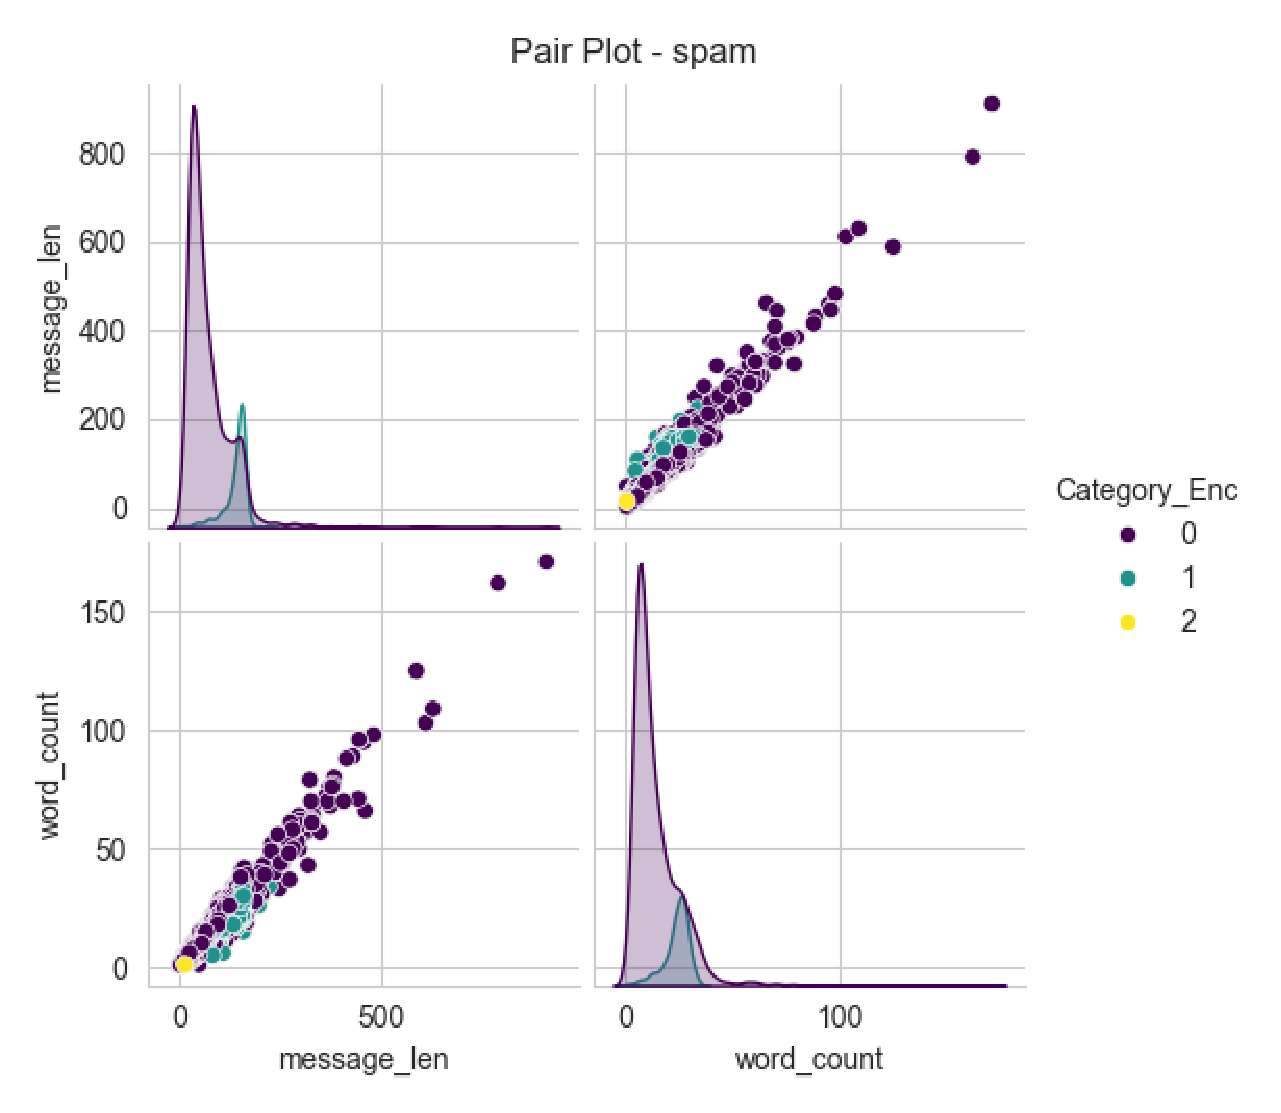
\includegraphics[width=0.45\linewidth]{image_eps/spam_pairplot.eps}
    \caption{Spam Dataset: Correlation Heatmap and Pair Plot}
\end{figure}

\subsection{MNIST / Digits Image EDA}
\begin{itemize}
    \item \textbf{Intensity Distribution:} Visualized using histograms of pixel intensities, showing most pixels are near-zero (background) with sharp peaks near 255 (stroke pixels).
    \item \textbf{Spatial Verification:} Visualized a $5 \times 5$ grid of digit samples to verify correct labeling and check for variations in handwriting styles.
    \item \textbf{Dimensionality:} Each $28 \times 28$ image was flattened, and the variance across features was assessed to ensure high information content.
\end{itemize}

\begin{figure}[H]
    \centering
    \includegraphics[width=0.45\linewidth]{image_eps/digits_hist.eps}
    \includegraphics[width=0.45\linewidth]{image_eps/digits_box.eps}
    \caption{Digits Dataset: Histograms and Box Plots}
\end{figure}
\begin{figure}[H]
    \centering
    \includegraphics[width=0.45\linewidth]{image_eps/digits_heatmap.eps}
    \includegraphics[width=0.45\linewidth]{image_eps/digits_pairplot.eps}
    \caption{Digits Dataset: Correlation Heatmap and Pair Plot}
\end{figure}

\section{Domain Methodology}
\subsection{Loan Prediction}
A \textbf{Random Forest Classifier} was used to predict loan status after handling missing values and categorical mapping for features like \texttt{Married} and \texttt{Education}.

\subsection{Diabetes Prediction}
Implemented \textbf{Logistic Regression} to determine diabetes probability, focusing on key contributors like \texttt{Glucose} and \texttt{BMI} as identified during the correlation analysis.

\subsection{Sequence-to-Sequence (NMT)}
Developed an \textbf{LSTM-based Encoder-Decoder} model to translate English phrases to Tamil, leveraging a context vector to transfer linguistic meaning across time steps.

\section{Conclusion}
The integration of systematic EDA with advanced machine learning models provided a holistic workflow for data science projects. EDA not only highlighted the inherent structure of the five datasets but also provided the necessary justification for pre-processing techniques and model selection.

\end{document}
